\documentclass[conference]{IEEEtran}
\usepackage{cite}
\usepackage{amsmath,amssymb,amsfonts}
\usepackage{algorithmic}
\usepackage{graphicx}
\usepackage{textcomp}
\usepackage{xcolor}
\usepackage{float}
\usepackage{tikz, pgfplots}
\usepackage{circuitikz}
\usepackage[english]{babel}
\usepackage[autostyle, english = american]{csquotes}
\MakeOuterQuote{"}
\def\BibTeX{{\rm B\kern-.05em{\sc i\kern-.025em b}\kern-.08em
    T\kern-.1667em\lower.7ex\hbox{E}\kern-.125emX}}

\pgfplotsset{compat=newest}

\begin{document}

\title{MSP432 Timers, Interrupts, and Analog-to-Digital Converter\\

\author{\IEEEauthorblockN{Tevin Hendess}
\IEEEauthorblockA{\textit{Computer Engineering Department} \\
\textit{Rochester Institute of Technology}\\
Rochester, NY USA \\
twh4619@rit.edu}
\and
\IEEEauthorblockN{Adam Schultzer}
\IEEEauthorblockA{\textit{Computer Engineering Department} \\
\textit{Rochester Institute of Technology}\\
Rochester, NY USA \\
ajs1539@rit.edu}
}
}

\maketitle

\begin{abstract}
An essential part of modern electronics is the ability to interact with
analog voltages that arise from sensors. Important parts of interpreting
these signals are using timers and ADCs (Analog to Digital Converters) to
sample the analog data into digital data. Demonstrating these concepts was
accomplished by enabling the proper peripherals on a MSP432 microcontroller,
these being the ADC and Timer32 modules, and programming the microcontroller
to sample temperature and light sensors, using the Timer32 module
as a clock, and the ADC to receive analog data. Data was processed and
visualized in tests to ensure that the analog sampling was performed as
expected. These tests utilized MatLab to visualize digital conversions,
which were compared to a waveform recorded on an oscilloscope.
\end{abstract}

\section{Design Methodology}

\subsection{Usage of Timers}
In order to accurately sample many external sensors, a clock signal must be 
used to synchronize the outputs of the sensor and the inputs of the ADC in
the microcontroller. Although a clock signal is necessary, the
microcontroller's internal clock would be a poor choice of a signal to use
for this purpose, as inputs would be received at the same pace that the
processor can execute instructions. Instead, timer interrupts were used to
reduce the main clock signal to a significantly slower and more usable
frequency. A Timer32 module of the MSP432 was used for this purpose.

The Timer32 module was used to generate interrupts at a rate of 2Hz and
1kHz, with the 2Hz signal being used to toggle an LED, and the 1kHz signal
being used to measure time between button presses in milliseconds. The 2Hz
signal was also used to trigger data collection from a temperature sensor,
so that the program would receive updated data two times a second.

% part 1 end

\subsection{Analog to Digital Conversion}
Before constructing the final form of the circuit which would take input from
a line-scan camera, a more simple ADC circuit was constructed. To practice
with analog to digital conversion, a temperature sensor was connected to the
MSP432 board via extension wires.

This sensor is much less complicated than a full 128 bit definition camera,
but still presented some challenges. The first was pulling the information
from the device via the ADC. This required code which would configure one of
the ADC clusters on the microcontroller to suit a temperature sensing
application. Two of the most important variables that had to be set were the
reference voltage (which was set at 2.5V according to information from the
MSP432 datasheet) and the interrupts which were completely disabled on the ADC
itself.

Though interrupts were used to obtain data from the ADC, the Timer32 module
was used as it interrupts at a set frequency rather than the ADC which will
interrupt whenever the it receives new data (which would have been far more
than required).
Once the raw data from the temperature sensor was converted to a digital value
through the ADC hardware, conversions had to be performed, this time in
software, to output a human-readable temperature in degrees Centigrade and
Fahrenheit. The equation for converting the raw digitized voltage to Celsius
is shown in Equation 1.

\begin{equation}
    Celsius = ((int) analogIn) / 142.46f - 10;
\end{equation}

In Equation 1, Celsius is the floating point variable storing the current
temperature in degrees Centigrade and analogIn is the direct digitized analog
input from the ADC. For these variables, it was very important that the types
be correct in order for the mathematical operations to perform as expected.
Celsius had to be a floating point value in order to store non-whole numbers
and analogIn had to be typecast into an integer rather than used in its
original, unsigned integer form. The two constants in Equation 1 come from the
temperature sensor datasheet which proclaims a range of the device between
10°C and 125°C. The maximum value was divided by the maximum voltage value of
the ADC (3.3V) to determine a scaling factor which was then applied to the
analog input. The subtraction of ten accounts for the range offset beginning
at 10°C rather than 0°C.

Once the value was expressed in degrees Centigrade, the conversion to
Fahrenheit was trivial and is shown in Equation 2.

\begin{equation}
    Fahrenheit = celsius * (9.0f/5.0f) + 32.0f;
\end{equation}

Because the celsius variable is already a floating point value, no special
typecasts need to be performed in Equation 2. The mathematical operations are
simply a direct conversion of degrees Centigrade to degrees Fahrenheit. First
multiplying by $\frac{9}{5}$ and then adding 32.

%Part 2 End

\subsection{Line Scan Camera}
Once the Timer32 module had been properly configured along with the ADC
circuitry, the two parts could be brought together to function as a
translation for the line scan camera.

This device outputs a 128 segment vector which contains the light level of
each segment. Using this, it is possible to detect dark spots and to create a
binary map of what the camera is seeing.

To create this, the setup was straightforward as the difficult portions were
configuring the Timer and ADC which had already been completed previously. The
camera had to be connected to the microcontroller with jumper wires which ran
3.3V, GND, CLK, SI, and AO.

Each of these signals served a different purpose and connected to a different
circuit in the microcontroller. 3.3V and GND provided the power to the camera
to actually take in data. CLK was connected to the SysTickTimer module which
was configured at 200Hz and was responsible for pulsing the camera rapidly. SI
is the scan signal and determines when the camera will actually scan in the
information. These two signals work together with the CLK pulsing 129 times
between each SI pulse which ensures that all of the segments are properly
scanned. Finally, the AO value is what the camera outputs as an analog signal
representing all segments in the scan.

The AO signal is the camera's only output and is what is connected to the
microcontroller's ADC for further processing. Some of this processing involves
Matlab code which smooths the signal and converts the fluctuations into a
simple digital output.

These two functions are relatively straightforward. Smoothing is done by
averaging every five bits of information which has the effect of limiting the
impact of outliers and providing for a more steady output overall. The binary
conversion examined the AO signal and used a threshold (determined in this
case to be 8000 as this is about half of the range of analog values) to
determine whether the value should be considered "light" (all values above the
threshold) or "dark" (everything below). This formula will need to be
rewritten every time the camera is introduced to a new environment in order to
account for different ambient light levels.

\section{Results and Analysis}

\subsection{Timer and Port Interrupts}

Before testing other systems, it was first necessary to test that the timer
modules were behaving as expected. To test the 2Hz timer interrupts, the
program was flashed onto the MSP432 development board and tested manually.
The intended behavior of a button enabling and disabling a LED to flash at
2Hz was demonstrated, showing the correct operation of the interrupts. To
test the 1kHz interrupts, a program was written to count an amount of
milliseconds between two presses of a button. This program output the amount
of time measured to a UART serial terminal when a second button press was
detected. This results of this test are shown in Fig.~\ref{part1terminal}.

\begin{figure}
    \centering
    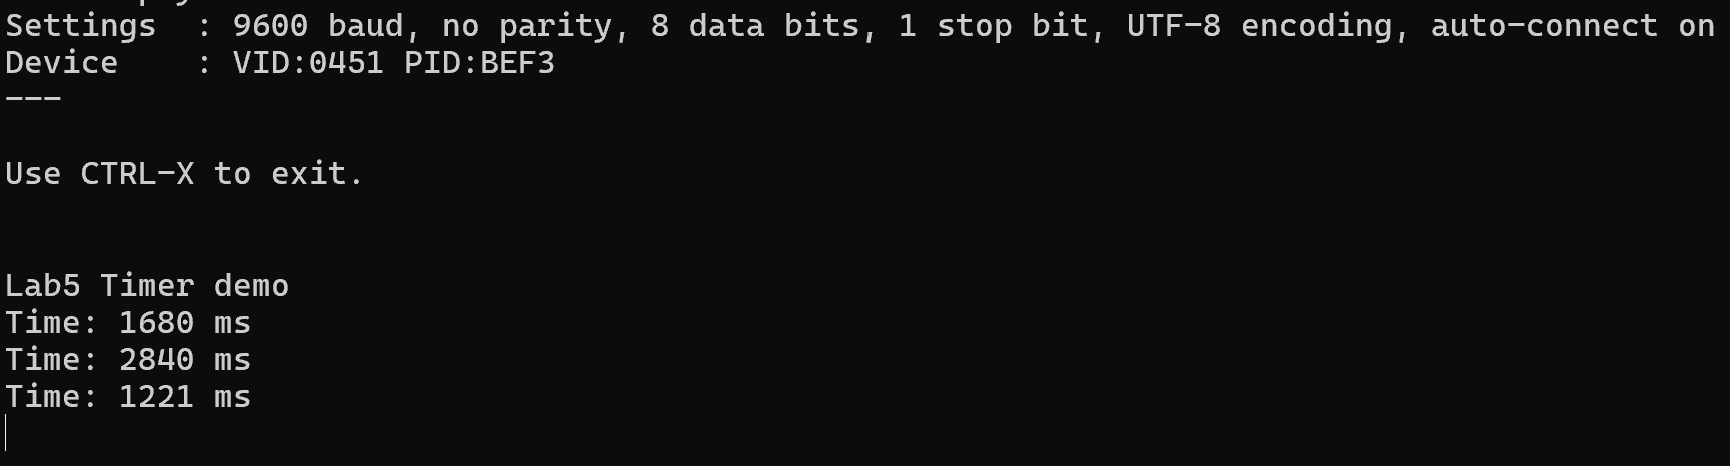
\includegraphics[width=\linewidth,decodearray={1 0 1 0 1 0}]{images/part1terminal.png}
    \caption{UART Output from Interrupt Testing}
    \label{part1terminal}
\end{figure}

These tests also confirmed that the port interrupts were functioning
correctly. The port interrupts were executed when the switches on the
MSP432 board were interracted with, allowing them to toggle the flashing
of the LED as well as telling the program when to start and stop the
counting of the 1kHz timer. Both of these functions were performed
successfully during these tests.

%end part 1

\subsection{ADC Temperature Sensor}

With the Timer32 module successfully verified, the analog to digital 
conversion also had to be checked. In this case, the algorithm to convert
analog voltages to degrees Centigrade and Fahrenheit wasn't the focus, though
this conversion had to be correct, but it was instead most pressing to
determine whether the ADC module had been configured correctly in terms of
inputs and interrupts. The terminal output resulting from connecting the
temperature sensor to the microcontroller and then converting and translating
the values is shown in Fig.~\ref{part2terminal}.

\begin{figure}
    \centering
    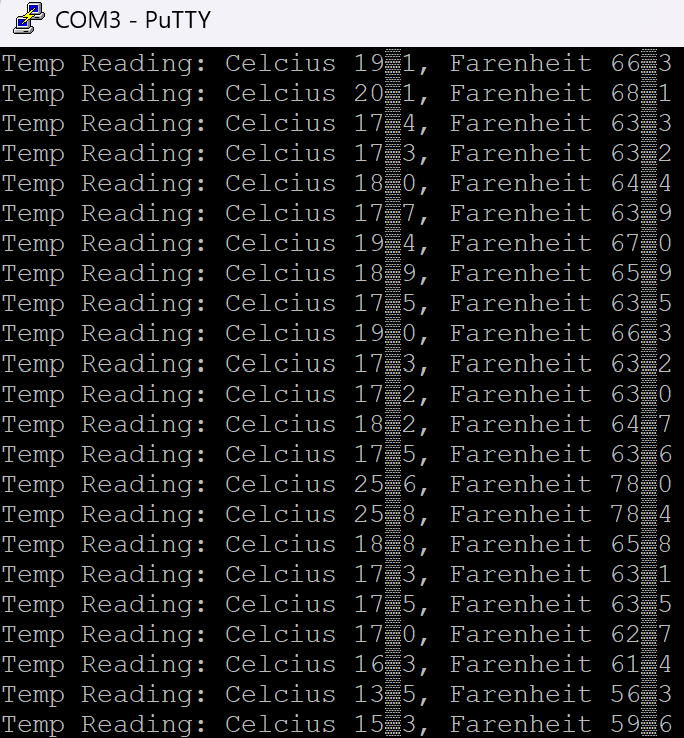
\includegraphics[width=\linewidth,decodearray={1 0 1 0 1 0}]{images/part2terminal2.png}
    \caption{UART Output from ADC Testing}
    \label{part2terminal}
\end{figure}

As displayed in Fig.~\ref{part2terminal}, the temperature according to the
sensor was displayed on the screen continuously every half second according to
the period of the timer module which flagged an interrupt that read from the
analog input.

The UART output was slightly incorrect as the "." character was not printing
properly within the terminal. This may have been a result of the floating
point values and how the print buffer was stored in a character array
variable. A discussion with experts on the matter determined that fixing the
issue was not feasible and stood beyond the scope of what was being tested.

\subsection{Camera Dark/Light Output Graphs}

With each of the smaller portions independently verified, the two could
finally be combined in the application of the line scan camera. This device
was tested in multiple ways to ensure that both the hardware and software
setups would produce the same, correct results. To determine the validity of
the hardware setup, the AO jumper wire was connected to an oscilloscope probe
rather than the ADC on the microcontroller. This way, the direct voltage value
could be read and it could be observed to be changing when the camera was
pointed at different shades. The result of this test is displayed in
Fig.~\ref{oscilloscope}

\begin{figure}
    \centering
    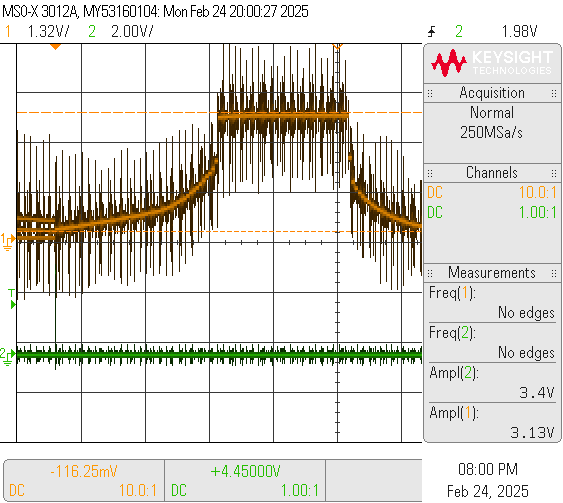
\includegraphics[width=\linewidth]{images/part3scope.png}
    \caption{Oscilloscope Capture of the Camera Voltage Output}
    \label{oscilloscope}
\end{figure}

The oscilloscope in Fig.~\ref{oscilloscope} displays two waveforms. The top
waveform is the actual voltage value coming from the camera which in this case
displays a peak in the center with two lower valleys on either side. This
waveform is indicative of what the camera was seeing which was a bright light
in the center, surrounded on both sides by a dark backdrop.

The second, lower line in Fig.~\ref{oscilloscope} is not exciting to look at
as any variations aren't noticeable, but it's inclusion is essential for the
proper analysis of the camera. This second probe was placed in line with the
SI input in such a way that the input was still able to reach the camera, but
could also be tracked on the oscilloscope. As SI is the signal which controls
when the camera should begin a new scan, setting the oscilloscope to also
start a new scan on a change in SI meant that the top waveform would match
perfectly with one full scan from the camera.

With the oscilloscope to test the hardware, a Matlab program was used to
verify the software and perform more complicated smoothing and binary
conversions, as previously discussed. The resulting Matlab graphs are shown in
Fig.~\ref{matlab}.

\begin{figure}
    \centering
    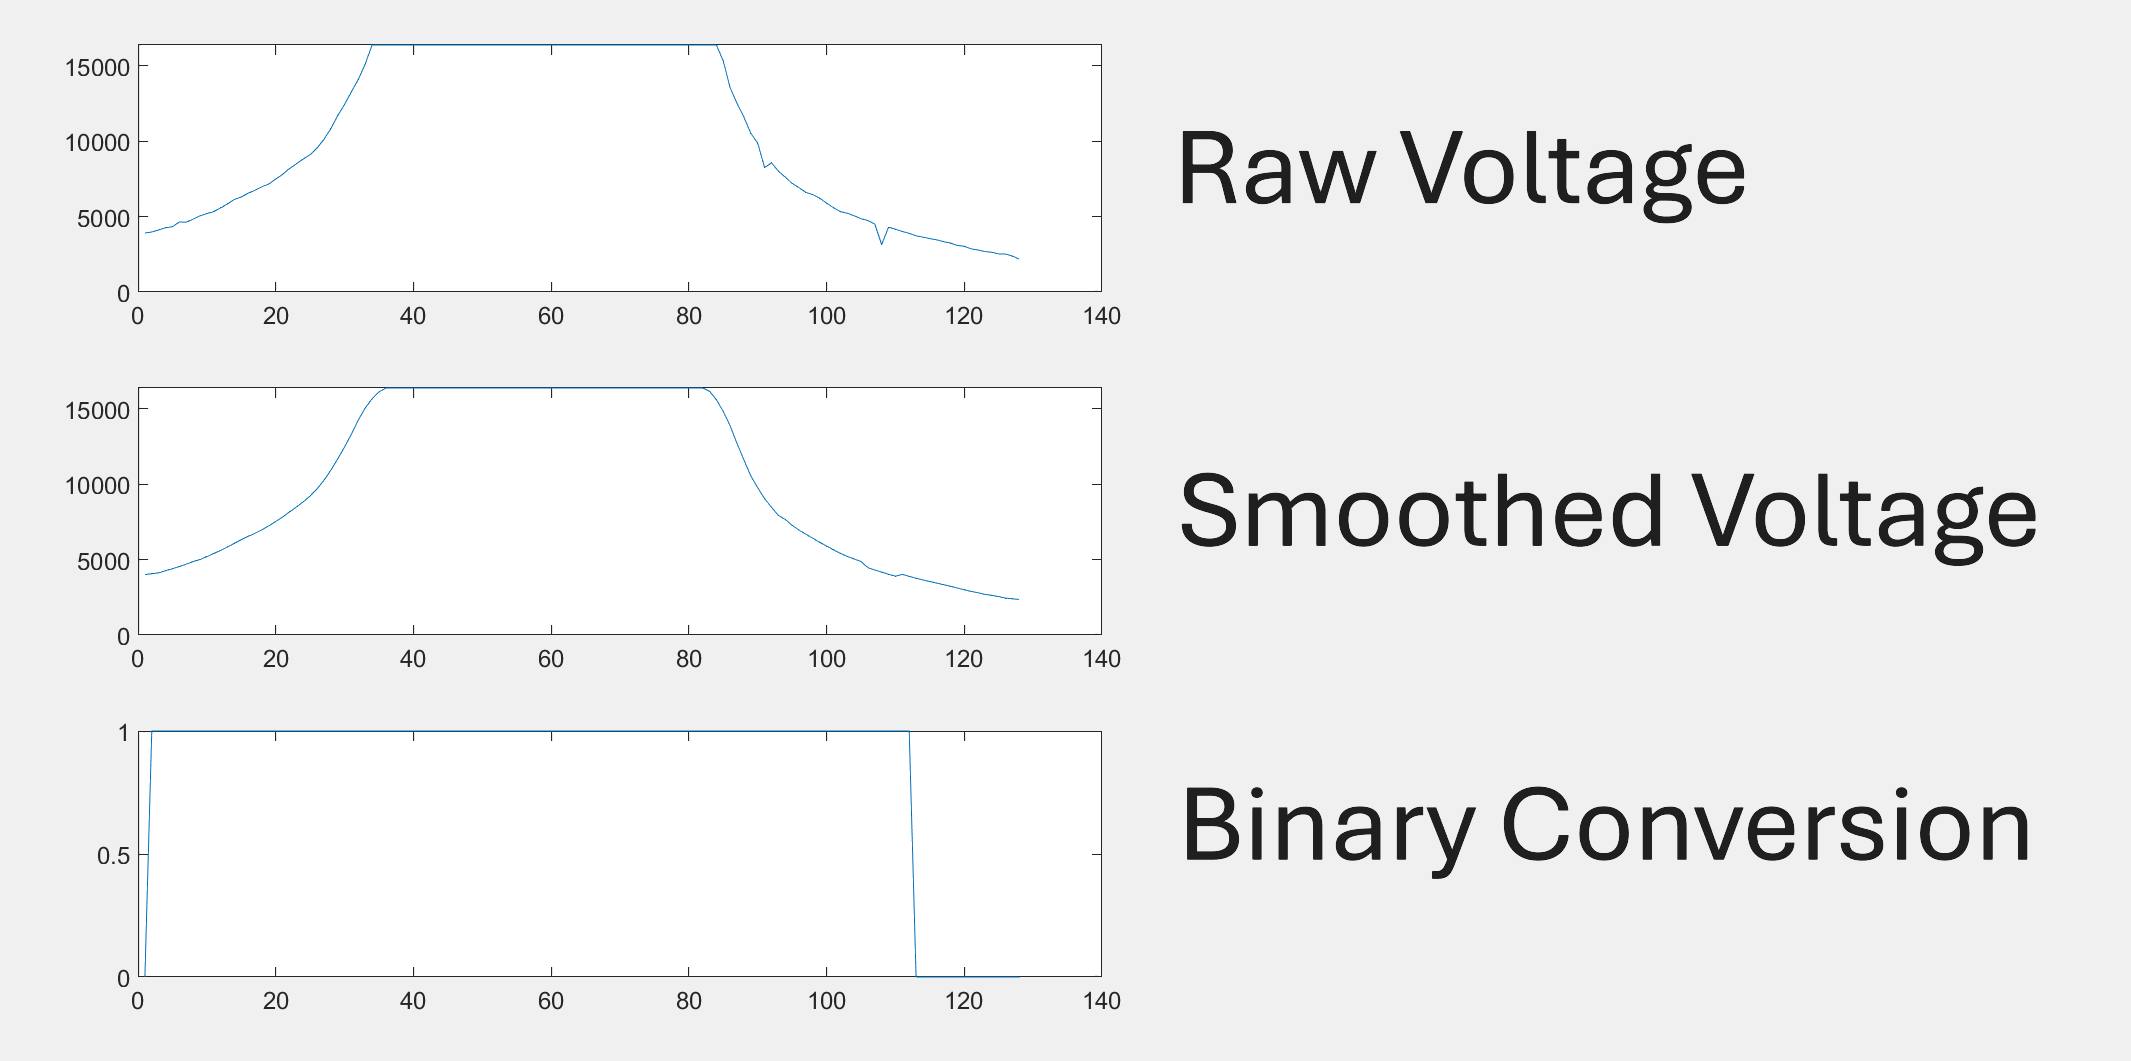
\includegraphics[width=\linewidth]{images/part3matlab.png}
    \caption{Matlab Graphs of the Camera Voltage Output}
    \label{matlab}
\end{figure}

The three graphs in Fig. ~\ref{matlab} are each a different step of the
simplification process. The top graph is the raw voltage which looks very
similar to that shown in Fig. ~\ref{oscilloscope} (the camera was pointed at
the same image). The smoothed voltage doesn't have quite as significant of
jumps in voltage, most notably at 90 and 110 where the dips displayed on the
raw graph have been completely smoothed over. Finally, the binary conversion
plot takes the voltage values and equates them to a binary "1" or "0"
depending on the threshold. Due to how the threshold was set, all values
before the second dip are considered high, while after that is low. As
previously mentioned, this threshold will need to be recalibrated (either
automatically or by hand) for each new environment that the camera is used for
every time it is used as even something as simple as the light from the sun
can change on different days and at different times.

\section{Questions}

\subsection{Why do the IRQ flags need to be cleared in the interrupt service
routine functions?}

The IRQ flags need to be cleared in the ISR function due to the fact that
these flags are the way that the NVIC (Nested Vectored Interrupt Controller)
keeps track of interrupt conditions and therefore which interrupts are pending 
and need to be executed. If a flag is not cleared, the ISR will be executed 
repeatedly, unless some other code or interrupt with a higher priority clears 
the flag.

\subsection{When an interrupt occurs, how do you know which pin caused it?}

In order to find what pin caused an interrupt, the IFG register of the port
that the interrupt came from can be checked. The pin that caused the
interrupt will have its respective bit of the IFG register set since it had
a pending interrupt. At the end of the ISR, it is essential to clear this
bit.

\subsection{What is the startup sequence of SI and CLK to initiate data 
transfer from the Camera?}

The clock signal, CLK, is used to latch the SI signal, and as such, the SI
signal must not be changed on a clock edge to aboid metastability. To
initiate a scan, SI goes high before the rising edge of the clock signal.
Once the rising edge arives, the SI signal must go low before the next
rising edge of the clock. This sequence starts a capture, and each subsequent
rising edge moves through a single pixel on the output. Eventually, the end
of the frame is reached, and SI must pulse high again in order to begin
another capture and data transfer.

\section{Conclusion}
Throughout the process of configuring a timer module, then an analog to 
digital converter, then finally combining the two for a camera, each step 
built upon the last and utilized elements which had been set up previously. 
Jumping straight to the camera would've been exceedingly difficult without the
 earlier testing completed and any issues with those components ruled out. The
camera's operation itself is also incredibly important to understand, both in 
how it gathers data and how to process that information. The line scan is a 
unique way of interpreting the world, but now that it is understood, along 
with how to simplify the information gathered into more actionable data, the 
camera can be successfully put to more advanced uses.

\end{document}
